%%%%%%%%%%%%%%%%%%%%%%%%%%%%%%% Inciso 01A:
$a$) \begin{lstlisting}
  {with {a { + 2 2 } }
    {with {b { + a a } }
      {with {foo { fun {x} {- x b } } }
        {with {a {- 2 2 } }
          {with {b {- a a } }
            {foo -3 } } } } }
\end{lstlisting}

Primero construyamos las pilas de ambientes, con
respecto al régimen de evaluación, esto es

\begin{multicols}{2}
  % Régimen Perezoso
  $*$) Con evaluación perzosa:
  \begin{center}
    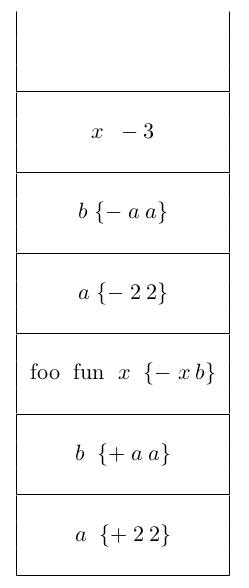
\includegraphics[scale=0.52]{./Perezosa}
  \end{center}

  \begin{enumerate}
  \item Evaluación perezosa y alcance estático.
  \begin{lstlisting}
  {foo -3 }
  {foo {x}{-x b}{-3}}
  {foo {x}{-x (+a a)}{-3}}
  {foo {x}{-(-3) (+a a)}}
  {foo {x}{-(-3) (+ (+2 2) a)}}
  {foo {x}{-(-3) (+ (+2 2) (+2 2))}}
  {foo {x}{-(-3) (+ (+2 2) (4))}}
  {foo {x}{-(-3) (+ (4) (4))}}
  {foo {x}{-(-3) (8)}}
  {-(-3) (8)}
  {-11}
  = -11

\end{lstlisting}
%%%%%%%%%%%%%%%%%%%%%%%%%%%%%%%%%%%%%%%%%%%%%%%%%%%%%
  \item Evaluación perezosa y alcance dinámico.
  \begin{lstlisting}
  {foo -3 }
  {foo {x}{-x b}{-3}}
  {foo {x}{-x (-a a)}{-3}}
  {foo {x}{-(-3) (-a a)}}
  {foo {x}{-(-3) (- (-2 2) a)}}
  {foo {x}{-(-3) (- (-2 2) (-2 2))}}
  {foo {x}{-(-3) (- (-2 2) (0))}}
  {foo {x}{-(-3) (- (0) (0))}}
  {foo {x}{-(-3) (0)}}
  {-(-3) (0)}
  {-3}
  = -3
  \end{lstlisting}
  \end{enumerate}

  \newpage
  % Régimen Glotón
  $*$) Con evaluación glotona:
  \begin{center}
    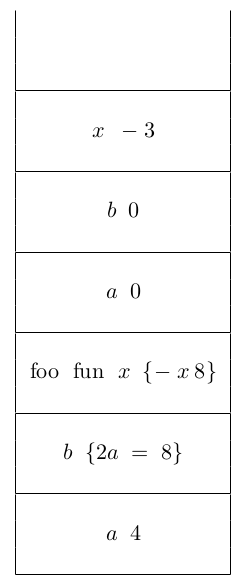
\includegraphics[scale=0.55]{./Glotona}
  \end{center}

  \begin{enumerate}
  \item Evaluación glotona y alcance estático.
  \begin{lstlisting}
  {foo -3 }
  {foo {x}{-x b}{-3}}
  {foo {x}{-x (8)}{-3}}
  {foo {x}{-(-3) (8)}}
  {-(-3) (8)}
  {-11}
  = -11
\end{lstlisting}

%%%%%%%%%%%%%%%%%%%%%%%%%%%%%%%%%%%%%%%%%%
  \item Evaluación glotona y alcance dinámico.
  \begin{lstlisting}
  {foo -3 }
  {foo {x}{-x b}{-3}}
  {foo {x}{-x (0)}{-3}}
  {foo {x}{-(-3) (0)}}
  {-(-3) (0)}
  {-3}
  = -3
\end{lstlisting}
  \end{enumerate}

\end{multicols}
